\section{Cyclic Processes with an Ideal Gas}

\begin{comment}
This lab is more of a worksheet than it is a lab.  But I've used versions of if in my 132 classes for a while, so I thought it was time to include it here in the lab manual for others as well.  --Matt Trawick, 6/2015

Activity 1 is straightforward practice with the ideal gas law, Q, E, and W.
Activity 2 works through isothermal and adiabatic expansions.
Activity 3 is the only part that actually works to introduce a new topic, as opposed to practicing something the students are presumed to have seen before.

In the past, I've done Activities 1 and 2 on different days, as two different worksheets.

\end{comment}

\makelabheader %(Space for student name, etc., defined in master.tex)

\vspace{0.1in}
\textbf{Objective} 

In this lab, you will examine an ideal gas going through a cycle in which it is compressed and expanded, eventually returning to its initial state.  During this time, thermal energy enters and leaves the gas, and useful work can be extracted from it.  These cycles are the basis of refrigerators (which put work into a system to move heat energy from something cold to something hot) and heat engines (which move heat energy from something hot to something cold, extracting useful work along the way.

\textbf{Activity 1: A Rectangular Cycle}

\begin{wrapfigure}[3]{r}{0.48\textwidth}
%    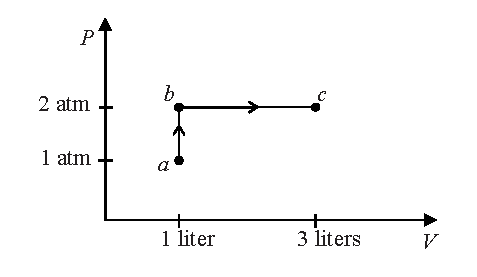
\includegraphics[width=0.4\textwidth]{ideal_gas_cycles/square_cycle1.eps}
\vspace{-0.2 in}
\hspace*{\fill}
\begin{lab_axis}[lab_noticks_1quad,
	algebraic_labels,
	width=2.1in, height=1.3in,	
	xmax=4, ymax=3,
	xlabel={$V$},
	ylabel={$P$},
	xtick={1,3},
	xticklabels={{1 liter}, {3 liters}},
	ytick={1,2},
	yticklabels={$1 \times 10^5$ Pa, $2 \times 10^5$ Pa},
	]
\addplot [path_leg] coordinates {(1,1)(1,2)};
\addplot [path_leg] coordinates {(1,2)(3,2)};
%\addplot [path_leg] coordinates {(3,2)(3,1)};
%\addplot [path_leg] coordinates {(3,1)(1,1)};
\addplot [path_point]  coordinates {(1,1)(1,2)(3,2)};
\node[anchor=north east] at (axis cs: 1,1)  {$a$};
\node[anchor=south east] at (axis cs: 1,2)  {$b$};
\node[anchor=south west] at (axis cs: 3,2)  {$c$};
%\node[anchor=north west] at (axis cs: 3,1)  {$d$};
\end{lab_axis}
\end{wrapfigure}

We start with a sample of 1 liter of nitrogen ($\textrm{N}_2$) gas, at temperature $T_a = 300$ K and pressure $P_a = 10^5$ N/m$^2$ (about 1 atm).

(a) Find the number of moles $n$ of the gas.
\answerspace{1.0in}

(b) As the figure shows, the gas is heated at constant volume from point $a$ to point $b$, then heated at constant pressure to point $c$.  Find the temperatures $T_b$ and $T_c$.  
\answerspace{1.4in}

(c) Find the change in the internal energy $E$ for the gas for the processes $a \rightarrow b$ and $b \rightarrow c$.  (Call these $\Delta E_{ab}$ and $\Delta E_{bc}$.)
\answerspace{1.5in}

\pagebreak
(d) Find the work done on the gas for each process, $W_{ab}$ and $W_{bc}$.  
\answerspace{1.3in}

(e) Find the heat added to the gas for each process, $Q_{ab}$ and $Q_{bc}$.  
\answerspace{1.3in}


\begin{wrapfigure}[3]{r}{0.45\textwidth}
\vspace{-0.2 in}
%  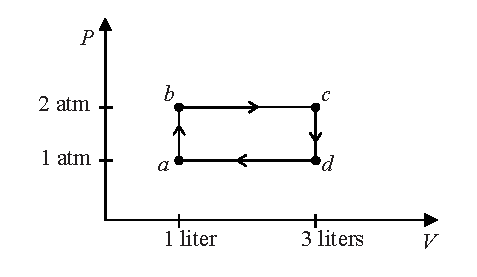
\includegraphics[width=0.4\textwidth]{ideal_gas_cycles/square_cycle2.eps}
\hspace*{\fill}
\begin{lab_axis}[lab_noticks_1quad,
	algebraic_labels,
	width=2.1in, height=1.3in,	
	xmax=4, ymax=3,
	xlabel={$V$},
	ylabel={$P$},
	xtick={1,3},
	xticklabels={{1 liter}, {3 liters}},
	ytick={1,2},
	yticklabels={$1 \times 10^5$ Pa, $2 \times 10^5$ Pa},
	]
\addplot [path_leg] coordinates {(1,1)(1,2)};
\addplot [path_leg] coordinates {(1,2)(3,2)};
\addplot [path_leg] coordinates {(3,2)(3,1)};
\addplot [path_leg] coordinates {(3,1)(1,1)};
\addplot [path_point]  coordinates {(1,1)(1,2)(3,2)(3,1)};
\node[anchor=north east] at (axis cs: 1,1)  {$a$};
\node[anchor=south east] at (axis cs: 1,2)  {$b$};
\node[anchor=south west] at (axis cs: 3,2)  {$c$};
\node[anchor=north west] at (axis cs: 3,1)  {$d$};
\end{lab_axis}
\end{wrapfigure}

Now the gas is cooled at a constant volume from point $c$ to point $d$, and cooled at constant pressure from point $d$ back to point $a$.  

(f) Find the temperature $T_d$ at point $d$.
\answerspace{1.5in}

(g) Complete the following table:

%For fixed width columns:
%These are now defined in master.text:
%\newcolumntype{L}[1]{>{\raggedright\arraybackslash}p{#1}}
%\newcolumntype{C}[1]{>{\centering\arraybackslash}p{#1}}
%\newcolumntype{R}[1]{>{\raggedleft\arraybackslash}p{#1}}

\vspace{0.1 in}
{\renewcommand{\arraystretch}{2.0}
\begin{tabular}{| C{1in} |C{1in} | C{1in} | C{1in} |}
\hline
& $\Delta E$ & $W$ & $Q$ \\ \hline
$a \rightarrow b$ & & & \\ \hline
$b \rightarrow c$ & & & \\ \hline
$c \rightarrow d$ & & & \\ \hline
$d \rightarrow a$ & & & \\
\hhline{|=|=|=|=|}
NET: & & & \\ \hline
\end{tabular}
}

\vspace{0.3in}

\pagebreak
\textbf{Activity 2: A Carnot Cycle}

As in the previous activity, we start with 1 liter of ($\textrm{N}_2$) gas at temperature $T_a = 300$ K and pressure $P_a=10^5$~N/m$^2$.   As you found before, this gives $nR=\frac{1}{3}$~J/K, or $n=0.0401$~moles.  We'll heat the gas to a maximum temperature of 1800 K again, but here we do so in one step, a single adiabatic compression, as shown in process $a \rightarrow b$ of the figure below.

%\begin{minipage}{0.44\textwidth}
%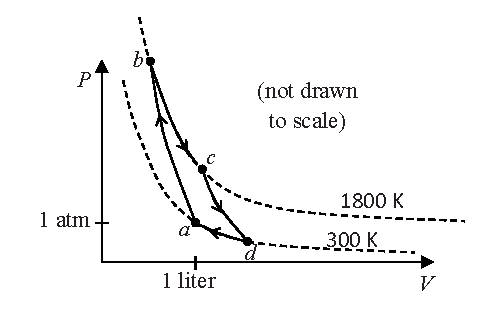
\includegraphics[width=1.0\textwidth]{ideal_gas_cycles/carnot_cycle.eps}
%\end{minipage}
%\begin{minipage}{0.54\textwidth}

\raisebox{-.5\height}{
\begin{lab_axis}[lab_noticks_1quad,
	algebraic_labels,
	width=2.3in, height=1.7in,	
	xmax=3.1, ymax=4.5,
	xlabel={$V$},
	ylabel={$P$},
	xtick={1},
	xticklabels={{1 liter},},
	ytick={1},
	yticklabels={$10^5$ Pa},
	]
\addplot [black,dashed,very thick, domain= 0.20 : 4] {1/x};
\addplot [black,dashed,very thick, domain= 0.25 : 2.4] {2/x};
%\addplot [black, domain= 0.25 : 4] {1/x^2};
%\addplot [black, domain= 0.25 : 4] {2.5/x^2};
\addplot [path_leg, domain= 1 : 0.5] {1/x^2};
\addplot [path_leg, domain= 0.5 : 1.25] {2/x};
\addplot [path_leg, domain= 1.25 : 2.5] {2.5/x^2};
\addplot [path_leg, domain= 2.5 : 1] {1/x};
\addplot [path_point]  coordinates {(1,1)(0.5,4)(1.25,1.6)(2.5,0.4)};
\node[anchor=north east] at (axis cs: 1,1)  {$a$};
\node[anchor=east] at (axis cs: 0.5,4)  {$b$};
\node[anchor=south west] at (axis cs: 1.25,1.6)  {$c$};
\node[anchor=north east] at (axis cs: 2.5,0.5)  {$d$};
\node[anchor=south west, rotate=-4] at (axis cs: 2.5,0.3)  {300 K};
\node[anchor=south east, rotate=-12] at (axis cs: 2.5,0.7)  {1800 K};
\node[anchor=north west, text width = 0.9in] at (axis cs: 1.5,4)  {(not drawn \\ to scale)};
\end{lab_axis}
} %end of raisebox
\hspace*{\fill}
{\renewcommand{\arraystretch}{2.0}
\begin{tabular}{| C{0.3in} | C{0.6in} | C{0.6in} | C{0.6in} | C{0.6in} |}
\hline
& $P$ & $V$ & $nR$ & $T$ \\ \hline
$a$ & $10^5$ Pa & $10^{-3}$ m$^3$ & $\frac{1}{3}$ J/K & 300 K \\ \hline
$b$ &                  &                            & $\frac{1}{3}$ J/K & 1800 K \\ \hline
$c$ &                  &                            & $\frac{1}{3}$ J/K & 1800 K \\ \hline
$d$ &                  &                            & $\frac{1}{3}$ J/K & 300 K \\ \hline
\end{tabular}}
%\end{minipage}

(a) Recalling that $PV^\gamma$ is constant for an adiabatic process, where $\gamma = C_P / C_V$, what is the final volume $V_b$?  (Hint: write $P_a V_a^\gamma = P_b V_b^\gamma$, and express both of the $P$'s in terms of $V$ and $T$. Answer: $V_b=1.134 \times 10^{-5}$ m$^3$.)  
\answerspace{2.2in}


(b) What are $\Delta E_{ab}$, $W_{ab}$, and $Q_{ab}$?  Go ahead and start filling out the table on the next page if you like.  Also, the table at the top of this page may help you keep your thoughts organized.
\answerspace{1.6in}

\pagebreak
(c) In the process $b \rightarrow c$, the gas is expanded isothermally to a new volume, $V_c=1.6918 \times 10^{-5}$ m$^3$.  (This particular value for $V_c$ makes the numbers in the table turn out pretty.  You'll see.)  Calculate $\Delta E_{bc}$, $W_{bc}$, and $Q_{bc}$ for this process.  
\answerspace{1.6in}

(d) Now the gas is expanded adiabatically back to $T_d=300$ K.  Find $V_d$, and also find  $\Delta E_{cd}$, $W_{cd}$, and $Q_{cd}$.
\answerspace{2.0in}


(e) Finally, the gas is compressed isothermally back to $V_a$.  Find $\Delta E_{da}$, $W_{da}$, and $Q_{da}$.  
\answerspace{1.6in}



(f) If you haven't done so already, complete the following table:
\vspace{0.1 in}

{\renewcommand{\arraystretch}{2.0}
\begin{tabular}{| C{1in} |C{1in} | C{1in} | C{1in} |}
\hline
& $\Delta E$ & $W$ & $Q$ \\ \hline
$a \rightarrow b$ & & & \\ \hline
$b \rightarrow c$ & & & \\ \hline
$c \rightarrow d$ & & & \\ \hline
$d \rightarrow a$ & & & \\
\hhline{|=|=|=|=|}
NET: & & & \\ \hline
\end{tabular}
}

\pagebreak
\textbf{Activity 3: Comparing the Two Cycles}

Both of the cycles you have just examined are examples of ``heat engines.''  In each case, some heat energy $Q_{\rm IN}$ enters the gas from an external source called the ``hot reservoir.''   Some of that heat energy, $Q_{\rm OUT}$, is expelled to a ``cold reservoir,'' and some is converted to work.    As an example, think of an electrical power plant that burns coal to make steam to drive a generator.  Heat energy flows from the hot burning coal to the water, some of which is expelled to the outside air through a smoke stack, and some of which is converted to useful work.

(a)  What is the total heat $Q_{\rm IN}$ that entered the gas from the hot reservoir in each of the two cycles you examined in activites 1 and 2?

\medskip
$\displaystyle
\hspace{0.5in} 
\left| Q_{\substack{\textrm{IN} \\ \\ \textrm{rect}}} \right| = \hspace{\fill}
\left| Q_{\substack{\textrm{IN} \\ \\ \textrm{Carnot}}} \right|= \hspace{\fill}
$
\answerspace{0.4in}

(b) What is the total heat $Q_{\rm OUT}$ dumped out of the gas into the cold reservoir in each cycle?

\medskip
$\displaystyle
\hspace{0.5in} 
\left| Q_{\substack{\textrm{OUT} \\ \\ \textrm{rect}}} \right| = \hspace{\fill}
\left| Q_{\substack{\textrm{OUT} \\ \\ \textrm{Carnot}}} \right|= \hspace{\fill}
$
\answerspace{0.4in}

(c)  What is the net work $W$ done by the gas in each cycle?  (That's work ``\textbf{by} the gas,'' not ``\textbf{on} the gas''.) 

\medskip
$\displaystyle
\hspace{0.5in} 
W_{\substack{\textrm{NET} \\ \\ \textrm{rect}}} = \hspace{\fill}
W_{\substack{\textrm{NET} \\ \\ \textrm{Carnot}}} = \hspace{\fill}
$
\answerspace{0.4in}

(d)  The ``thermal efficiency'' $\eta$ of the heat engine is defined as the ratio of the work done to the heat energy in.  Calculate the thermal efficiency for each of the two cycles.

\medskip
$\displaystyle
\hspace{0.5in} 
\eta_{\rm rect} = \hspace{\fill}
\eta_{\rm Carnot} = \hspace{\fill}
$
\bigskip

(e) If the two cycles you studied were power plants, which one would generate the most electrical energy per ton of coal burned, and why?





